\documentclass{article}


\usepackage{PRIMEarxiv}

\usepackage[utf8]{inputenc} % allow utf-8 input
\usepackage[T1]{fontenc}    % use 8-bit T1 fonts
\usepackage{hyperref}       % hyperlinks
\usepackage{url}            % simple URL typesetting
\usepackage{booktabs}       % professional-quality tables
\usepackage{amsfonts}       % blackboard math symbols
\usepackage{nicefrac}       % compact symbols for 1/2, etc.
\usepackage{microtype}      % microtypography
\usepackage{fancyhdr}       % header
\usepackage{graphicx}       % graphics
\usepackage{float}
\graphicspath{{media/}}     % organize your images and other figures under media/ folder

%Header
\pagestyle{fancy}
\thispagestyle{empty}
\rhead{ \textit{ }} 

% Update your Headers here
\fancyhead[LO]{deep routing lab}
% \fancyhead[RE]{Firstauthor and Secondauthor} % Firstauthor et al. if more than 2 - must use \documentclass[twoside]{article}



  
%% Title
\title{Deep Routing Lab
% %%%% Cite as
% %%%% Update your official citation here when published 
% \thanks{\textit{\underline{Citation}}: 
% \textbf{Authors. Title. Pages.... DOI:000000/11111.}} 
}

\author{
  Jonathan M. Frame \\
  University of Alabama \\
  Department of Geological Sciences \\
  Tuscaloosa, AL\\
  \texttt{\{jmframe\}@ua.edu} \\
  %% examples of more authors
}


\begin{document}
\maketitle


\begin{abstract}
Deep Routing Lab is a codebase designed for hydrologists to build an intuition for using geospatial machine learning methods. This lab includes examples of training a convolutional neural network on synthetic data representing digital terrain, dynamic storm precipitation and terrain routing. The trained network represents a toy (surrogate) model of routing water from precipitation-driven flow across a terrain. 
\end{abstract}


\section{Introduction}
Hydrologists are increasingly working with machine learning, deep learning, neural networks and all sorts of artificial intelligence. There is a need for improving the education for undergraduates and graduate students of hydrology. We've previously offered the deep bucket lab for developing skills and intuition for time series modeling in hydrology. Here we offer the routing lab for skills and intuition for geospatial modeling in hydrology. Geospatial modeling is useful for many applications of remote sensing, and for general movement of water around the globe. 

Applications of geospatial modeling in hydrology are not as popular as time series modeling. 

Much research has been done for these types of AI applications \cite{behroozi2025sensitivity}. This lab follows the theoretical reasoning for the flood inundation mapping by \cite{frame2024rapid}.

\section{Convolution as a geospatial model}
\label{sec:conv}
Convolutional networks, especially those with multiple layers and skip connections, have the ability to pass information from the input data to the target prediction at various scales and at various distances within the modeling domain. This makes them ideal for geospatial hydrological modeling because hydrological responses depend on phenomena that occurs at a variety of scales and distances. They work well on images, and for a long time were the gold standard of image processing, and this also makes them ideal for geospatial modeling, since the majority of our environmental and hydrological data comes in the form of images, either portraying input variables like temperature, or relevant data from satellites.

\section{Simple CNN examples}
\label{sec:simple}

This section introduces students to convolutional neural networks (CNNs) through two self-contained examples. Both examples use synthetic image data, where the task is to predict the pixel-wise product of two input images. This setup is intentionally simple to isolate and explore how CNNs learn spatial relationships and perform pixel-wise operations.

\subsection{Monolith example in Jupyter notebook}
\label{sec:mono}

The monolithic example is implemented as a single Jupyter notebook (\texttt{MONO\_notebook\_simpleCNN1.ipynb}). It combines data generation, model definition, training, and evaluation in a single script. This format helps students:
\begin{itemize}
    \item Understand each step of the machine learning workflow in a linear, top-down fashion.
    \item See how synthetic image data can be used to learn spatial transformations.
    \item Trace how a CNN propagates and transforms information through convolution, pooling, and dense layers.
    \item Experiment with architecture choices like filter size, hidden dimensions, and learning rate.
\end{itemize}

By working through this notebook, students gain an intuitive understanding of:
\begin{itemize}
    \item What a CNN is doing at each layer.
    \item How two separate image inputs are encoded, fused, and decoded into a spatial prediction.
    \item How network depth and nonlinearity influence model capacity, even for a simple pixel multiplication task.
\end{itemize}

\subsection{A cleaner setup for deep learning}
\label{sec:clean}

To build better coding habits and prepare for more complex tasks, a modular version of the same CNN is also included. This setup separates responsibilities into multiple files:
\begin{itemize}
    \item \texttt{cnn\_model.py}: CNN architecture
    \item \texttt{data\_generation.py}: Synthetic data creation and preprocessing
    \item \texttt{train\_model.py}: Model training loop
    \item \texttt{evaluate\_model.py}: Visualization and performance evaluation
    \item \texttt{config.py}: Centralized parameter definitions
\end{itemize}

This modular structure reflects standard practice in research and production ML pipelines. By working through this version, students learn:
\begin{itemize}
    \item How to organize a deep learning project into reusable components.
    \item How to configure experiments using shared parameter files.
    \item How evaluation and visualization are integrated into a learning workflow.
\end{itemize}

Together, the monolithic and modular versions provide complementary experiences. The monolithic version helps students understand CNN behavior at a conceptual level, while the modular version prepares them to scale up to real-world, maintainable research code.

\subsubsection{Excercise: Modify the target process}
\label{sec:simpleexcercise}

In the simple CNN examples, the model is trained to reproduce the result of a predefined function that transforms two input images, $x_1$ and $x_2$, into a target image $y$. This transformation is defined in the function \texttt{SYSTEM\_PROCESS}, which currently computes the element-wise product:

\begin{verbatim}
def SYSTEM_PROCESS(x1, x2):
    return x1 * x2
\end{verbatim}

This provides a useful but simple task for the network: it must learn to identify how each pixel in the output corresponds to the multiplication of the matching pixels in the two inputs.

Try replacing it with a different operation in \texttt{SYSTEM\_PROCESS}, such as:
\begin{itemize}
  \item \texttt{(x1 + x2) / 2}
  \item \texttt{np.maximum(x1, x2)}
  \item \texttt{np.sin(x1) + np.cos(x2)}
\end{itemize}

Retrain the model and observe how the network adapts to different target behaviors.

\section{The Source Code}
\label{sec:src}

Most of the lab work takes place in \texttt{src/dr/}, which includes modules for generating synthetic data, training a convolutional network, and plotting results—similar to the simple CNN example, but now with more realistic (though fictional) hydrologic responses.

To enable full functionality, run \texttt{pip install .} from the project root. 

\section{Synthetic terrain generation}
\label{sec:terrain}
The synthetic terrain is generated using the code in \texttt{src/drl/dem\_generator.py}, which includes a stochastic simulator that evolves a digital elevation model (DEM) over time. It begins with low-frequency noise to represent broad elevation patterns and iteratively adds smooth perturbations to simulate natural terrain variability. At each iteration, the DEM is modified by one of three operations: strong smoothing, light smoothing, or river carving. These introduce realistic topographic features while maintaining a controlled elevation range.

The river carving algorithm emulates erosion by starting from a random edge point and cutting a shallow path across the DEM, simulating flow-driven terrain modification. All DEMs are clipped at the edges to avoid boundary artifacts. This approach produces varied but hydrologically plausible terrain samples that can be used as input to routing and CNN models.

\section{Synthetic storm generation}
\label{sec:storm}

Rainfall inputs are generated using the simulator in \texttt{src/drl/rain\_generator.py}. Each storm is modeled as a Gaussian rainfall pulse that travels across the DEM in a randomly chosen cardinal direction (north, south, east, or west). Key parameters such as intensity, speed, and spread (sigma) are sampled randomly within user-defined ranges.

The storm moves one step per timestep, depositing rainfall in a spatially distributed pattern centered along its path. The simulator supports generating storms in a single direction or in all four directions using consistent storm parameters, enabling controlled comparisons in routing experiments.

\section{Hyrdaulic Routing}
\label{sec:routing}

Surface water movement is simulated using a diffusive wave approximation implemented in \texttt{src/drl/overland\_router.py}. The model uses explicit time stepping to compute water depth changes over a digital elevation model (DEM) in response to rainfall. It accounts for topographic slopes, Manning's roughness, and gravitational acceleration to calculate overland flow.

Rainfall is applied as a time-varying input, and water routing proceeds with adaptive sub-timesteps to satisfy the CFL condition for numerical stability. At each step, water fluxes between cells are computed based on hydraulic gradients, and divergence of those fluxes is used to update local water depth. The model stores the evolving water depth fields for later analysis or comparison with predictions.

\section{Generating Training Data}
\label{sec:datagen}

Synthetic training data is generated using \texttt{src/drl/data\_generator\_parll.py}. Each sample consists of a digital elevation model (DEM), a sequence of rainfall snapshots, and a corresponding water depth field computed from hydraulic routing.

For each sample, the pipeline performs the following steps: (1) generate a random DEM, (2) simulate a storm over that terrain, (3) compute the resulting water depths using the diffusive wave router, and (4) extract rainfall snapshots leading up to a randomly selected timestep. These components are saved both as compressed NumPy arrays and as visualization-ready PNG images.

To run the generator:
\begin{verbatim}
python src/drl/data_generator_parll.py --config config/config.yaml --out_dir dataset/
\end{verbatim}

This script uses all available CPU cores to parallelize the process and create a large training set efficiently.

\section{Deep Routing Emulator}
\label{sec:deeprouting}

To accelerate hydraulic simulations, we introduce a deep learning emulator that learns to reproduce the behavior of the routing model. Instead of computing water depth through numerical integration of physical equations, this model predicts the final depth field directly from the initial terrain and rainfall inputs. This approach enables faster predictions while maintaining spatial accuracy.

The model takes as input a digital elevation map (DEM) and a sequence of rainfall snapshots leading up to a specific timestep. These are stacked along the channel dimension and passed to a convolutional network, which outputs a single-channel image representing the predicted water depth at that timestep. See Figure~\ref{fig:model_io} for an illustration of the model's input–output structure.

\begin{figure}[H]
    \centering
    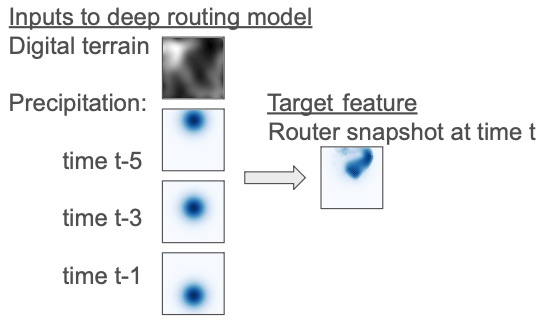
\includegraphics[width=0.85\textwidth]{fig/modelio.png}
    \caption{Schematic of the deep routing emulator input and output. The model receives a DEM and multiple rainfall snapshots as input channels, stacked along the channel dimension. It outputs a single-channel map representing predicted water depth at a future timestep.}
    \label{fig:model_io}
\end{figure}

\subsection{Architecture}
\label{sec:arch}

The emulator is implemented in \texttt{src/drl/deep\_router.py} as a U-Net-style convolutional neural network. The network consists of a multi-scale encoder–decoder structure with skip connections and residual decoder blocks. It takes multi-channel geospatial input (e.g., stacked DEM and rainfall images) and outputs a single-channel map of predicted water depth.

The architecture is designed to capture both local and global spatial patterns in the input, making it well-suited for emulating the effects of terrain, rainfall intensity, and spatial water routing without iterative time stepping.

\subsection{A computational shortcut}
\label{sec:comp}

The task of the deep routing model is to learn a shortcut: given several rainfall inputs at discrete times and a terrain map, predict the final depth of inundation without simulating the full time evolution. The physical routing model integrates fine-scale processes over many small time steps, constrained by numerical stability and resolution. The emulator replaces this with a single forward pass.

This compression of physical evolution into an instantaneous transformation echoes what Wolfram describes as a computational reduction—finding a simpler rule that produces the same outcome as a more complex one~\cite{wolfram2023second}. Here, the deep model aims to approximate a snapshot state of a dynamical system through learned structure, rather than explicit simulation.

%Bibliography
\bibliographystyle{unsrt}  
\bibliography{references}  


\end{document}
